\chapter{Background}\label{chapter:background}
In this chapter, we will provide an overview of the key concepts and theories that are relevant to our work. We will also mention key background 
literature related to this work.

\section{Linguistics}
Linguistics, the scientific study of languages is a broad and complex field encompassing various subfields. Although a comprehensive summary 
of Linguistics is beyond the scope of this thesis, we will briefly discuss some of the subfields and key concepts that are relevant to our work.
\cite{trask2007language} provides a glossary of linguistic terms that can be useful for readers interested in a more detailed overview of the field.

\subsection{Phonetics and Phonology}
\textbf{Phonetics} is the study of the physical sounds of human speech, their production, transmission and reception. \cite{trask2007language}. 
The International Phonetic Alphabet (IPA) is a standardized system of phonetic notation that represents the sounds of spoken language. The system
is based on the assumption that speech can be represented partly as a sequence of discrete sounds or \textit{segments} \cite{handbookIPA1999}. 
In addition, the IPA also includes symbols for suprasegmental features such as stress and intonation. The full IPA Chart (reproduced here in 
\ref{fig:ipa_chart}) shows all the symbols and diacritics used to represent sounds in the IPA. Sounds and words can be transcribed in IPA 
using \textipa{[ ]} brackets. For example, the sounds for the word \textit{this} can be transcribed as \textipa{[DIs]}. The IPA helps linguistics
transcribe sounds in a language-agnostic way, allowing them to compare sounds across languages. The IPA Handbook \cite{handbookIPA1999} provides
a comprehensive guide to the use of the IPA.

\textbf{Phonology} is the study of the sound systems of languages, including the patterns of sounds and the rules that govern their distribution. \cite{trask2007language}.
The key difference in the disciplines is driven by the concept of a \textit{phoneme}. A phoneme is an abstract unit of sound that can distinguished
by a native speaker of a language. Phonemes and Phonemic transcriptions are represented using slashes \textipa{/ /}. The key points about phonemes are:
\begin{enumerate}
    \item Letters do not necessarily correspond to phonemes. For example, the English word \textit{this} has four letters but 3 phonemes (\textipa{/DIs/}).
    \item Phonemes can be realized as different sounds in different contexts. For example, the English phoneme \textipa{/p/} can be realized as
    \textipa{[p\super{h}]} in the word \textit{pin}(\textipa{[p\super{h}In]}) and \textipa{[p]} in the word \textit{spin}(\textipa{[spIn]}).
    i.e. in English, the sounds \textipa{[p]} and \textipa{[p\super{h}]} are \textit{allophones} of the phoneme \textipa{/p/}.
    \item Two sounds are considered different phonemes if changing them can change the meaning of a word. e.g. \textipa{[dEn]} \textit{den} and 
    \textipa{[DEn]} \textit{then} are distinct words in English.
\end{enumerate}

% From Wikipedia : In phonetics, the smallest perceptible segment is a phone. In phonology, there is a subfield of segmental phonology that deals with the 
% analysis of speech into phonemes (or segmental phonemes), which correspond fairly well to phonetic segments of the analysed speech.
% Also diff between segments and phonemes and phones?
% Should datasets like Phoible be mentioned here?

\textbf{Phonotactics} defines the rules that govern the permissible sound sequences in a language \cite{trask2007language}. For example, in English,
the sequence \textipa{/bl/} is permissible at the beginning of a word (e.g. \textit{bled}) but not the sequence \textipa{/bn/}. Languages usually
modify loadwords to fit their own phonotactic constraints. For example, the English word \textit{beer} is borrowed into Japanese as \textit{biru}.


\subsection{Morphology}
\textbf{Morphology} is the study of the structure of words and the rules that govern the formation of words in a language \cite{trask2007language}.
Most studies of morphology focus on the concept of a \textit{morpheme}, the smallest unit of meaning in a language. For example, the word \textit{unhappiness}
can be broken down into three morphemes: \textit{un-}, \textit{happy} and \textit{-ness}. Morphemes can be free or bound. Free morphemes can stand
alone as words (e.g. \textit{happy}) while bound morphemes must be attached to other morphemes (e.g. \textit{-ness}).

Morphology can be further divided into \textbf{inflectional} and \textbf{derivational} morphology. \textbf{Inflectional morphology} involves the
modification of a word for grammatical purposes such as tense, aspect, mood, number, e.g. the English verb \textit{walk} can be inflected to
\textit{walked}, \textit{walks}, \textit{walking}, etc. \textbf{Derivational morphology} involves the creation of new words from existing words.
For example, the English noun \textit{happiness} can be derived from the adjective \textit{happiness} by adding the suffix \textit{-ness}.

\subsubsection{Lexicon}
The \textbf{lexicon} of a language is the vocabulary of a language, i.e. the total set of words available for a speaker. It is better to consider
the lexicon, not as a list of word, but a set of lexical resources including morphemes, and processes to construct words from these resources \cite{trask2007language}.

\subsection{Grammar}
\textbf{Grammar} is the set of rules that govern the structure of sentences in a language. Traditional Grammar describes certain terms for basic
grammatical components such as \textit{article}, \textit{adjective}, \textit{noun}, etc known as \textit{parts of speech} \cite{yule2020StudyLanguage}.

\begin{enumerate}
    \item \textbf{Nouns} are words that refer to people, places, things, or abstract ideas, as if they were objects. For example, \textit{cat}, \textit{house}, and \textit{happiness} are all nouns.
    \item \textbf{Verbs} are words that express the actions or states of nouns. For example, \textit{run}, \textit{is}, and \textit{happen} are all verbs.
    \item \textbf{Adjectives} are words that describe or modify nouns. For example, \textit{happy}, \textit{red}, and \textit{tall} are all adjectives.
    \item \textbf{Adverbs} are words that describe or modify verbs, adjectives, or other adverbs. For example, \textit{really}, \textit{very}, and \textit{well} are all adverbs.
    \item \textbf{Articles} are words that define a noun as specific or unspecific. For example, \textit{the} is a definite article, while \textit{a} and \textit{an} are indefinite articles.
    \item \textbf{Pronouns} are words that take the place of noun phrases, typically when they are already known. For example, \textit{he}, \textit{she}, and \textit{they} are all pronouns.
    \item \textbf{Prepositions} are words that show the relationship between a noun or pronoun and other words in a sentence. For example, \textit{in}, \textit{on}, and \textit{at} are all prepositions.
    \item \textbf{Conjunctions} are words that connect words, phrases, or clauses, and indicate the relationship between them. For example, \textit{and}, \textit{but}, and \textit{or} are all conjunctions.
\end{enumerate}

Sometimes, parts of speech exhibit multiple forms, used in different grammatical circumstances. Each of these forms indicate a certain \textit{grammatical category} 
or \textit{feature}. For example, in English, verbs can be inflected for tense, aspect, mood, person, number, etc. This is known as \textit{agreement}.

A language may choose to explicitly mark these features, i.e. \textit{grammaticalize} them \cite{rosenfelder2010language}. All features can be
expressed in any language (perhaps by adding explicit information), but every language chooses to express only a subset of these features grammatically.

\subsection{Grammatical Features}
Grammatical features or categories provide some extra information about the sentence, and different parts of speech may exhibit different forms
to indicate these features. we will briefly discuss some of the most common grammatical features.

\subsubsection{Grammatical Gender}
In many languages, nouns are often classified into different classes, and different parts of speech will often agree with the specific class. These classes
are called Grammatical Gender, and it often need not have anything to do with sex or gender. Languages with gender may only have 2 gender classes, but can also
have many more. The gender assignment of many objects are often arbitrary. 

\subsubsection{Grammatical Number}
\textbf{Grammatical Number} is a grammatical category that expresses count distinctions. The most common distinction is between singular (one) and plural (many), but
some languages also have dual (two), trial (three), paucal (few), and other forms. For example, in English, the noun \textit{cat} is singular, while \textit{cats} is plural.

\subsubsection{Grammatical Case}
The \textbf{Grammatical Case} indicates one or more functions of a noun or noun phrase in a sentence. Many different cases have been identified in the worlds languages, such as

\begin{enumerate}
    \item \textbf{Nominative} case, which indicates the subject of a verb.
    \item \textbf{Accusative} case, which indicates the direct object of a verb.
    \item \textbf{Dative} case, which indicates the indirect object of a verb.
    \item \textbf{Genitive} case, which indicates possession.
    \item \textbf{Locative} case, which indicates location.
    \item \textbf{Instrumental} case, which indicates the means by which an action is performed.
\end{enumerate}
These descriptions are not exact, and precise distinctions can heavily depend on the specific language.

\subsubsection{Tense, Aspect and Mood}

Tense, aspect and modality all provide some kind of information that is temporal in nature, or tell us about the status of the action or verb. 
They are often grouped together as \textbf{TAM} (Tense, Aspect, Modality). 

\textbf{Tense} is a grammatical category that indicates the time at which an action takes place. The most common tenses are past, present, and future. 
For example, in English, the verb \textit{walk} can be inflected to \textit{walked} (past), \textit{walks} (present), and \textit{will walk} (future).


\textbf{Aspect} is a grammatical category that indicates the temporal structure of the action or event described by a verb. It indicates for example, 
whether the action is bounded, and unitary, or continuous or habitual. For example, in English, the sentences \textit{She danced} and \textit{She was dancing}
have different aspects. They are both in the past tense, but the first sentence indicates a \textit{perfective}, or completed aspect, while 
the second sentence indicates an \textit{continuous}, or \textit{progressive} aspect.

\textbf{Modality} is a grammatical category that indicates the speaker's attitude towards the action or event described by a verb. Modern linguists 
usually associate it with the expression of obligation, permission, prohibition, necessity, possibility and ability \cite{trask2007language}. In English,
modality is primarily expressed using Auxiliary verbs, such as \textit{can}, \textit{may}, \textit{must}, etc. For example, the sentence \textit{He can dance} indicates ability, while
the sentence \textit{He must dance} indicates obligation.


\subsubsection{Grammatical Person}
\textbf{Grammatical Person} is a grammatical category that indicates the different relationships between the speaker, the listener, and others in the discourse.
Languages typically indicate this relationship using pronouns. The most common distinctions are between first person (the speaker), second person (the listener), and third person (others).
For example, in English, the pronouns \textit{I} (first person), \textit{you} (second person), and \textit{he/she/they/it} (third person) indicate the grammatical person.

Some languages also have a distinction in \textit{clusivity} for the first person plural pronoun. The inclusive form includes the listener, while the exclusive form does not.
For example in Malayalam, the pronoun \textit{nammal} includes the listener, while the pronoun \textit{njangal} does not.

\subsection{Syntax}
\textbf{Syntax} is the study of the structure of sentences and the rules that govern the formation of sentences in a language \cite{trask2007language}.
The goal of Syntactic Analysis is to have a finite set of rules that could be used to generate potentially infinite sentences. This set of rules is known as 
a \textbf{Generative Grammar} \cite{yule2020StudyLanguage}. We move from the concepts of Nouns to Noun Phrases, and Verbs to Verb Phrases, and so on.

A Noun Phrase is a phrase that is interchangeable with a noun. Take for example the sentence:

\begin{center}
    \underline{\hspace{2cm}} bought a new car.
\end{center}

The cloze in the sentence could be filled with a noun, like "John", but also by say , "The young man".

With these definitions in mind, we could define a sentence as a Noun Phrase followed by a Verb Phrase. We can also have production rules for 
Noun Phrases, Verb Phrases, and so on. For example, a Noun Phrase could be defined as a determiner followed by an adjective followed by a noun.
With these rules, known as \textbf{Phrase Structure Rules}, we can generate a tree structure for a sentence, known as a \textbf{Parse Tree} \cite{jm3}.

%  TODO: Figure for Parse tree example + Description. see https://tex.stackexchange.com/questions/111196/how-to-create-syntactic-trees-and-align-them-in-latex
\begin{figure}
    \centering
    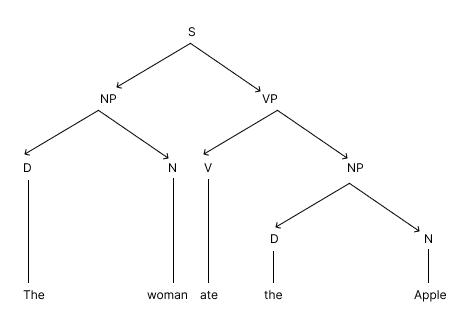
\includegraphics[width=0.8\textwidth]{figures/syntactic_parse_tree.png}
    \caption{Parse Tree for the sentence \textit{The woman ate the Apple}}
    \label{fig:parse_tree}
\end{figure}


\section{Constructed Languages}
Constructed Languages are languages that have not naturally evolved, but were artifically constructed. Some conlangs are created for fictional word-building,
like \textit{Quenya} and \textit{Sindarin} from J.R.R. Tolkien's Middle-Earth, or \textit{Dothraki} and \textit{High Valyrian} from George R.R. Martin's A Song of Ice and Fire.
Others are created for international communication, like \textit{Esperanto} and \textit{Volapük}. Some conlangs are created to be more logical or efficient, like \textit{Lojban} and \textit{Ithkuil}
, or easy to learn, like \textit{Toki Pona}.

Although people have been likely creating languages since time immemorial, \textit{Lingua Ignota}, created by the nun Hildegard von Bingen in 12 CE \cite{schreyerConstructedLanguages2021}.
Language Creation became popularized in the mainstream by J.R.R. Tolkien, who created several languages for his works, and his technique has influenced
many conlangers since \cite{petersonArtLanguageInvention2015}. In the early 90s, the internet allowed for the formation of a community of conlangers, 
who share their work and techniques online.

\subsection{The Process of Language Creation}

There has been a strong online community of language creators, called conlangers since the 1990s \cite{petersonArtLanguageInvention2015}. 
The community has created a wealth of resources for language creation. In particular, \cite{petersonArtLanguageInvention2015} and \cite{rosenfelder2010language} provide 
a comprehensive overview of the process of language creation. The process starts with the creation of a phonetic inventory, and phonotactics, which gives the language a distinct
character. The next steps involve, word building, grammar, semantics and pragmatics \cite{rosenfelder2010language}.


\section{Evaluation}
\subsection{Evaluation of Machine Translations}
Evaluation of machine translations is a complex task, and is essential for assessing the accuracy and fluency of the translations. Human evaluations
are often expensive and time-consuming \cite{papineniBLEUMethodAutomatic2002}, and are not always feasible for large datasets. As a result, many researchers 
have developed automatic evaluation metrics to assess the quality of machine translations. Classic methods like BLEU \cite{papineniBLEUMethodAutomatic2002} measures
the similarity between the machine translation and a reference translation by comparing n-grams. ROUGE \cite{linROUGEPackageAutomatic2004} is another popular metric that
measures recall as opposed to precision. It is often used for evaluating the quality of summaries, but can also be used for machine translation evaluation. METEOR \cite{banerjeeMETEORAutomaticMetric2005} 
improves upon such methods by for example, considering synonyms and stemming. 

We use these machine translation evaluation metrics by comparing the detranslated text with the original text. Although the actual values for these metrics would be
dependent on the model and its parameters, it would still be useful to compare the performance between different generated conlangs. 

\subsubsection{BLEU: Bilingual Evaluation Understudy} 
\textbf{BLEU} (Bilingual Evaluation Understudy) \cite{papineniBLEUMethodAutomatic2002} is one of the most widely used automatic metrics for 
evaluating machine translations. It measures the similarity between a machine translations and reference translations by analyzing their \textit{n-gram} overlap. The BLEU score is given by:

\begin{equation}
\text{BLEU} = \text{BP} \cdot \exp\left(\sum_{n=1}^{N} w_n \log p_n \right)
\end{equation}

where  $p_n$ is the geometric average of the precision of n-grams,  $w_n$ are weights assigned to different n-grams, and  $\text{BP}$ (the brevity penalty) 
penalizes short translations to prevent artificially high scores. BLEU focuses primarily on precision but does not consider recall or semantic meaning.

\subsubsection{ROUGE: Recall-Oriented Understudy for Gisting Evaluation}
ROUGE (Recall-Oriented Understudy for Gisting Evaluation) \cite{linROUGEPackageAutomatic2004} is a set of metrics primarily used for text summarization but 
also applicable to machine translation. Unlike BLEU, which focuses on precision, ROUGE focuses on recall, i.e. how much of the reference translation appears in the generated text. 
The most common variant, ROUGE-N, computes the recall of n-gram matches:

\begin{equation}
\text{ROUGE-N} = \frac{\sum_{s \in \text{ref}} \sum_{gram_n \in s} \text{count}_{match}(gram_n)}{\sum_{s \in \text{ref}} \sum_{gram_n \in s} \text{count}(gram_n)}
\end{equation}

Another variant, ROUGE-L, measures the longest common subsequence (LCS) between the reference and candidate translations, capturing 
fluency better. ROUGE is especially useful for evaluating translations with different word orders but similar meanings.

\subsubsection{METEOR: Metric for Evaluation of Translation with Explicit ORdering}
METEOR (Metric for Evaluation of Translation with Explicit ORdering) addresses some of BLEU's limitations by incorporating recall, stemming, synonym matching, and word order penalties. 
METEOR aligns words between candidate and reference translations using exact matches, stemmed matches, and synonym matches. The metric is computed as:

\begin{equation}
\text{METEOR} = F_{mean} \cdot (1 - Penalty)
\end{equation}

where $ F_{mean} $ is the harmonic mean of precision and recall, and $\text{Penalty}$ reduces the score for word order mismatches. METEOR can correlate better with human judgments than BLEU 
due to its ability to consider semantic variations.


\subsection{Information Theoretic Evaluation of Languages}
Natural language, being a means of communication consists primarily of information transmission \cite{debowskiInformationTheoryLanguage2020}. There have
been several attempts to quantify the information content of a language using information theory. Shannon \cite{shannonPredictionEntropyPrinted1951} introduced a new
method of estimating the entropy and in turn the redundancy of a language. Entropy in a sense measures the average amount of information for each letter in a text.
Natural language however, is not a minimal length source code. It operates under the constraints of incremental language processing, which enforces
systematicity, compositionality and concatenation as means of combination  \cite{futrellInformationTheoryBridge2022}. Redundancy often serves another
important purpose, which is to help in error correction and understanding in noisy environments \cite{gibsonHowEfficiencyShapes2019}.

\subsection{Reading Comprehension Evaluation of Language Models}
One of the primary goals of Natural Language Processing is teaching computers to read and understand the meaning of text. Reading comprehension 
thus presents itself as a suitable benchmark to evaluate a model's language understanding ability \cite{zengSurveyMachineReading2020}.  The goal 
of a reading comprehension task is to require the model to read one or more text passages and then answers questions about them. 

MRC tasks are generally classified into four categories. 
\begin{enumerate}
    \item \textbf{Cloze Style} tasks require the model to fill in the blanks in a passage. 
    \item \textbf{Multiple-Choice} tasks require the model to select the correct answer from a set of options.
    \item \textbf{Span Prediction} tasks require the model to extract a span of text from the passage that answers the question.
    \item \textbf{Freeform} tasks require the model to generate a free-form answer to the question.
\end{enumerate}

In our work, we decided to use Multiple-Choice tasks as a proxy for evaluating the constructed language. By evaluating the dataset on a model,
first with the original passage and then with the detranslated passage, we get a proxy measure for the information loss in the translation process.
Although some of this loss may be due to the model's inability to understand the constructed language, we can still use this for comparative 
analysis of different constructed languages.

\subsubsection{RACE-C Dataset}
The RACE-C Dataset \cite{liangNewMultichoiceReading2019} is a large-scale reading comprehension dataset based on college english exams from China.
It improves upon the previous RACE dataset \cite{laiRACELargescaleReAding2017} by providing a more challenging set of questions and answers. 
It consists of 4275 passages and 14122 questions. Figure~\ref{fig:race-c-sample} shows a sample article and question from the dataset.

%  Figure showing a random question from Race-C
\begin{figure}[htbp]
	\centering
	\begin{tcolorbox}[colback=gray!5!white, colframe=black]
		\small
		People have been painting pictures for at least 30,000 years. The earliest pictures were painted by people who hunted animals. They used to paint pictures of the animals they wanted to catch and kill. Pictures of this kind have been found on the walls of caves in France and Spain. No one knows why they were painted there. Perhaps the painters thought that their pictures would help them to catch these animals. Or perhaps human beings have always wanted to tell stories in pictures.
		
		.
		.
		.
		
		These days, we can write down a story, or record information, without using pictures. But we still need pictures of all kinds: drawing, photographs, signs and diagrams. We find them everywhere: in books and newspapers, in the street, and on the walls of the places where we live and work. Pictures help us to understand and remember things more easily, and they can make a story much more interesting.
		\vspace{0.5em}

		\textbf{Question:} Pictures of animals were painted on the walls of caves in France and Spain because \underline{\hspace{3cm}}.
		
		\textbf{Options:}
		\begin{itemize}
			\item[A.] the hunters wanted to see the pictures
			\item[B.] the painters were animal lovers
			\item[C.] the painters wanted to show imagination
			\item[D.] the pictures were thought to be helpful
		\end{itemize}
		
		\textbf{Correct Answer:} D
	\end{tcolorbox}
	\caption{Sample Article and Comprehension Question from RACE-C}
	\label{fig:race-c-sample}
\end{figure}

\subsection{Zipf's Law}
In 1935, George Zipf made an observation which he claimed to be a universal property of human languages: The more frequent a word, the 
shorter it tends to be \cite{kanwalZipfsLawAbbreviation2017}. This is known as \textbf{Zipf's Law of Abbreviation}, or simply \textbf{Zipf's Law}.

In mathematical terms,
\begin{equation}
    f(r) \propto \frac{1}{r^\alpha}
\end{equation}

Where $f(r)$ is the frequency of the $r^{th}$ most frequent word, and $\alpha$ is a constant known as \textit{Zipf's Exponent}. For natural languages,
the value of $\alpha$ is noted to be around $1$.

\section{Language Models and Embeddings}

\subsection{Representation Learning}
The performance of NLP tasks, or any machine learning tasks in general is dependent on the choice of data representation \cite{bengioRepresentationLearningReview2014}.
Classical methods often involve pain-stakingly hand-crafting features for each task, which is often not feasible for large datasets. \textbf{Representation learning}
presents a way to automatically learn representations from the data, which can then be used for various downstream tasks. 

Coming specifically to NLP, Words that occur in similar contexts tend to have similar meanings \cite{harrisDistributionalStructure1954}. This is 
known as the \textbf{Distributional Hypothesis}. This hypothesis is the basis for \textbf{Vector Semantics}, the idea of representing words as a point
in a high-dimensional space, where the distance between points represents the semantic similarity between words \cite{jm3}. These vectors are called 
\textbf{embeddings}. This idea has been extended to subword units \cite{wuGooglesNeuralMachine2016}, sentences, and even larger pieces of text.

Embeddings can be broadly classified into two categories: \textbf{static} and \textbf{contextual} embeddings. Static embeddings, such as 
Word2Vec \cite{mikolovDistributedRepresentationsWords2013} or GloVe \cite{penningtonGloVeGlobalVectors2014} are fixed representations
for each word, regardless of the context in which they appear. For example, the word \textit{bank} would have the same representation in both the sentences
\textit{I went to the bank to deposit money} and \textit{The river bank was flooded}. Contextual embedding methods like ELMo \cite{petersDeepContextualizedWord2018}, BERT \cite{devlinBERTPretrainingDeep2019}, 
and GPT-3 \cite{brownLanguageModelsAre2020}, on the other hand, create dynamic representations that depend on the context in which the word appears.

% TODO: add figure showing example of word embeddings in 2D space.

\subsection{Large Language Models}
In NLP, Language Modeling aims to model the generative likelyhood of word sequences to to predict the probabilities of the next or missing word
in a sequence \cite{zhaoSurveyLargeLanguage2025}. Traditionally, language models were based on the markov assumption, predicting the next word 
in a sequence based on the previous $n$ words, and they were called $n$-gram models \cite{jm3}. Neural Language Models, on the other hand, use neural networks
to learn the probability distribution of the next word in a sequence, and are trained on large corpora of text. Initially they were based on recurrant neural networks
such as LSTMs \cite{hochreiterLongShortTermMemory1997}, but have since evolved to use transformer architectures \cite{vaswaniAttentionAllYou2023}.

The transformer architecture is based on the self-attention mechanism, which allows the model to weigh the importance of different tokens in a sequence
when making predictions. This allows the model to capture long-range dependencies and relationships between tokens, which is crucial for 
understanding natural language. These models are often called Pre-trained Language Models (PLMs) because they are initially trained on large corpora of text,
called \textit{pre-training}, and then \textit{fine-tuned} on specific tasks, such as machine translation or reading comprehension. Researchers have noted that increasing the size of these models and the amount of training data leads to better performance on a wide range of NLP tasks, leading to the
rise of what are called \textbf{Large Language Models} (LLMs) \cite{brownLanguageModelsAre2020}.

% TODO: Introduce GPT, BERT, DeepSeek.
% More on fine tuning, perplexity etc.


\subsection{Clustering Algorithms}
\textbf{Clustering} can be defined as the task of grouping a set of objects in such a way that objects in the same group are more similar to 
each other than to those in other groups \cite{jainDataClustering502010}. There have been several clustering algorithms proposed in the literature,
including K-Means \cite{lloydLeastSquaresQuantization1982}, DBSCAN \cite{esterDensitybasedAlgorithmDiscovering1996}, and HDBSCAN \cite{campelloDensityBasedClusteringBased2013}.

Clustering algorithms can be broadly classified into two categories: \textbf{partitional} and \textbf{hierarchical} clustering \cite{jainDataClustering502010}. 
hierarchical clustering algorithms recursively find nested clusters, in either a bottoms-up or top-down fashion. Partitional clustering algorithms, on the other hand,
find all clusters in a single pass and do not create a hierarchy.

\section{WordNet}
In order to facilitate our pipeline with proper embeddings, We use WordNet \cite{millerWordNetLexicalDatabase1994}, a large lexical database of English.
WordNet groups words into sets of synonyms called \textit{synsets}, and provides short definitions and usage examples. It also records the
various semantic relations between these synonym sets.

\begin{figure}
    \centering
    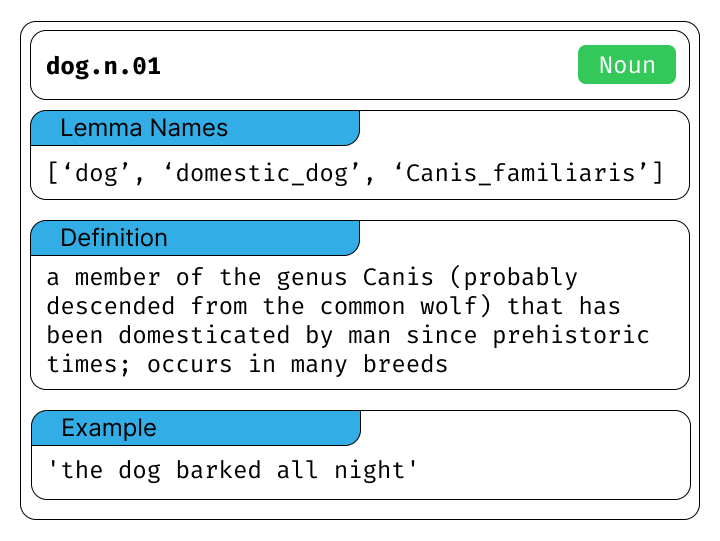
\includegraphics[width=0.8\textwidth]{figures/wordnet_single_synset.png}
    \caption{WordNet synset for the word \textit{dog.n.01}.}
    \label{fig:wordnet_single_synset}
\end{figure}

WordNet does not just interlink word forms, but specific senses of each word, which provides a more fine-grained representation of meaning.

\begin{figure}
    \centering
    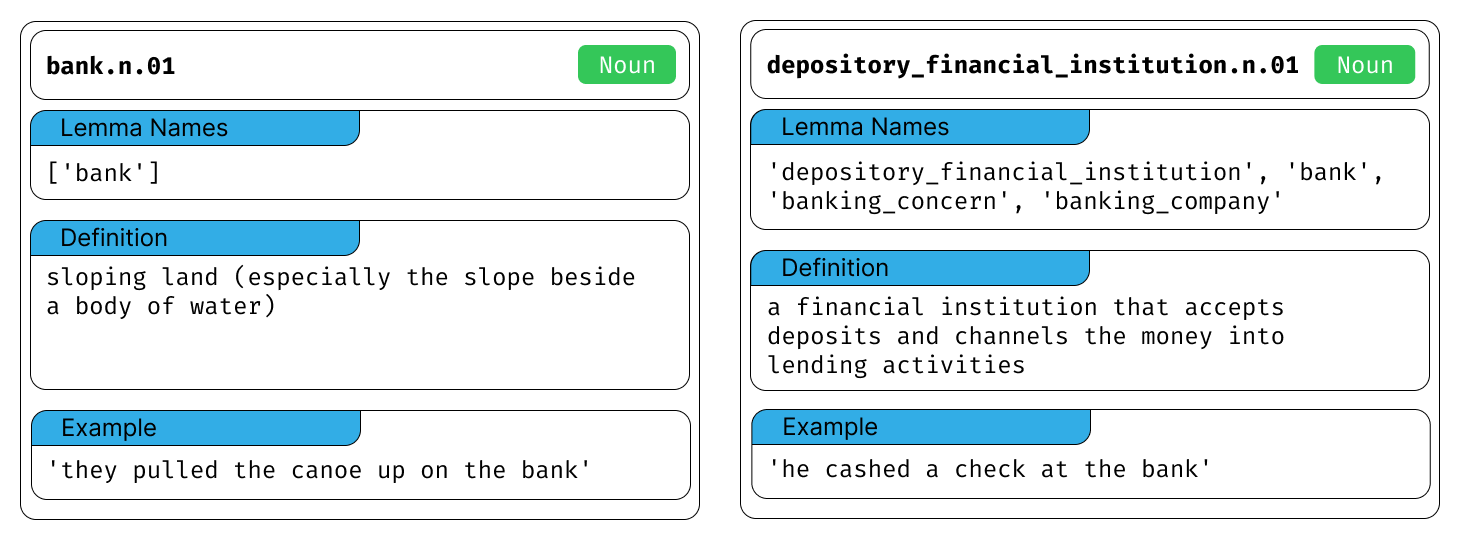
\includegraphics[width=0.8\textwidth]{figures/wordnet_multiple_synset.png}
    \caption{Comparing two senses for the word \textit{bank}.}
    \label{fig:wordnet_multiple_synset}
\end{figure}



